\subsection{On-Card Teil}
\label{subsec:3.2}
Der On-Card Teil wird durch das Applet $Traincard$ repräsentiert.
\\


Im Klassendiagramm in der Abbildung \ref{diaoncard} ist das Applet mit dessen Klassenvariablen und Methoden dargestellt.
Das Applet befindet sich im package\\htwk.smartcard.traincard und muss auf der verwendeten Smartcard installiert und gestartet werden.
\\

Entsprechend der Oberklasse javacard.framework.Applet, existieren Methoden, welche die Installation, Ausführung und Deselektion behandeln.
Die wichtigste Methode ist dabei process, welche ankommende APDUs erhält, diese auswertet, die entsprechende Klassenmethode aufruft und deren Antwort-Bytes in Form einer Response APDU zurücksendet.

\begin{figure}[htb]
\begin{center}
 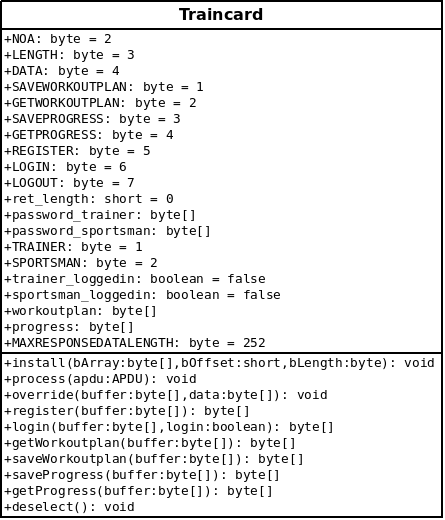
\includegraphics[width=.7\hsize]{./images/Klassendiagramm_oncard.png}
\end{center}
\caption[Klassendiagramm On-Card Teil]{\label{diaoncard}Klassendiagramm On-Card Teil}
\end{figure}


%das applet empfängt anfragen, wertet diese aus und sendet Daten oder ein erfolgsbyte im datenbereich zurück
%Daten werden dabei immer als byte arrays geschrieben und gelesen

%passwörter sind gehashed abgelegt

Das Instruktionsbyte wird mit den statischen Konstanten verglichen und anhand eines Treffers die entsprechende Methode aufgerufen. Jede dieser Methoden erhält den Puffer der APDU und gibt ein Byte Array für den Puffer der Response APDU zurück.
Der Aufbau der Command und Response APDU ist in der Abbildung \ref{myapdu} dargestellt.
Die darin dargestellten Data Bytes sind entsprechend der jeweiligen Instruktion gefüllt.\\
$00$ $02$ $01$ $01$ $01$ als APDU liest beispielsweise den Trainingsplan und sendet ihn zurück. Ist der Trainingsplan größer als MAXRESPONSEDATALENGTH Byte, muss mit $00$ $02$ $01$ $01$ $02$ eine weitere APDU mit den nächsten Bytes des Trainingsplanes angefordert werden.
\\

Lokale Byte Arrays der Methoden werden stets flüchtig mit der Methode makeTransientByteArray der Klasse javacard.framework.JCSystem angelegt.
Der Vergleich und das Kopieren von Byte Arrays erfolgt mit den Methoden arrayCompare und arrayCopy der Klasse javacard.framework.Util.
Dadurch wird der EEPROM der Smartcard nicht durch Schreibvorgänge belastet und die Ausführungszeit verringert sich.
\\

Der Trainingsplan und der Fortschritt wird in dynamischer Größe auf der Smartcard gespeichert und bei jedem Schreibvorgang neu erzeugt.